\indent En los siguientes tests queremos observar que sucede con cada familia de casos al ir variando los parámetros de entrada F, C de manera creciente y lineal y tomando los tiempos de corrida de cada input para poder compararlos.\\
Se comienza, por lo tanto, con una entrada de F*C = N y se la aumenta en cada test en una fila y columna hasta llegar a una matriz de 50*50. De manera que no hay desigualdades y todas las familias se miden en instancias de igual tamaño.\\
El origen siempre estará en la primer columna posible y el destino en la última. A medida que la matriz crezca, las posiciones de los mismos no serán alteradas y la cantidad de paredes y como varie el $P_{max}$ en cada caso, serán acordes para que siempre se encuentren dentro de la misma familia.\\

Para obtener dichas instancias se realizaron aproximadamente unas 20 corridas con el mismo input y se tom\'o el promedio de esas 20 corridas en cada instancia para obtener un valor m\'as cercano a la media.\\ 

Se pueden observar en el  gráfico 2.1, cinco funciones, que representan el tiempo de ejecuci\'on de las familias de casos mencionadas en el apartado anterior:

\begin{enumerate}
\item No existe árbol que conecte todas las salas
\item Existe un camino que conecta todas las salas de esfuerzo 0
\item El AGM es todo el grafo
\item Sin ejes
\item Camino por las salas random
\end{enumerate}

\vspace*{0.3cm} \vspace*{0.3cm}
  \begin{center}
 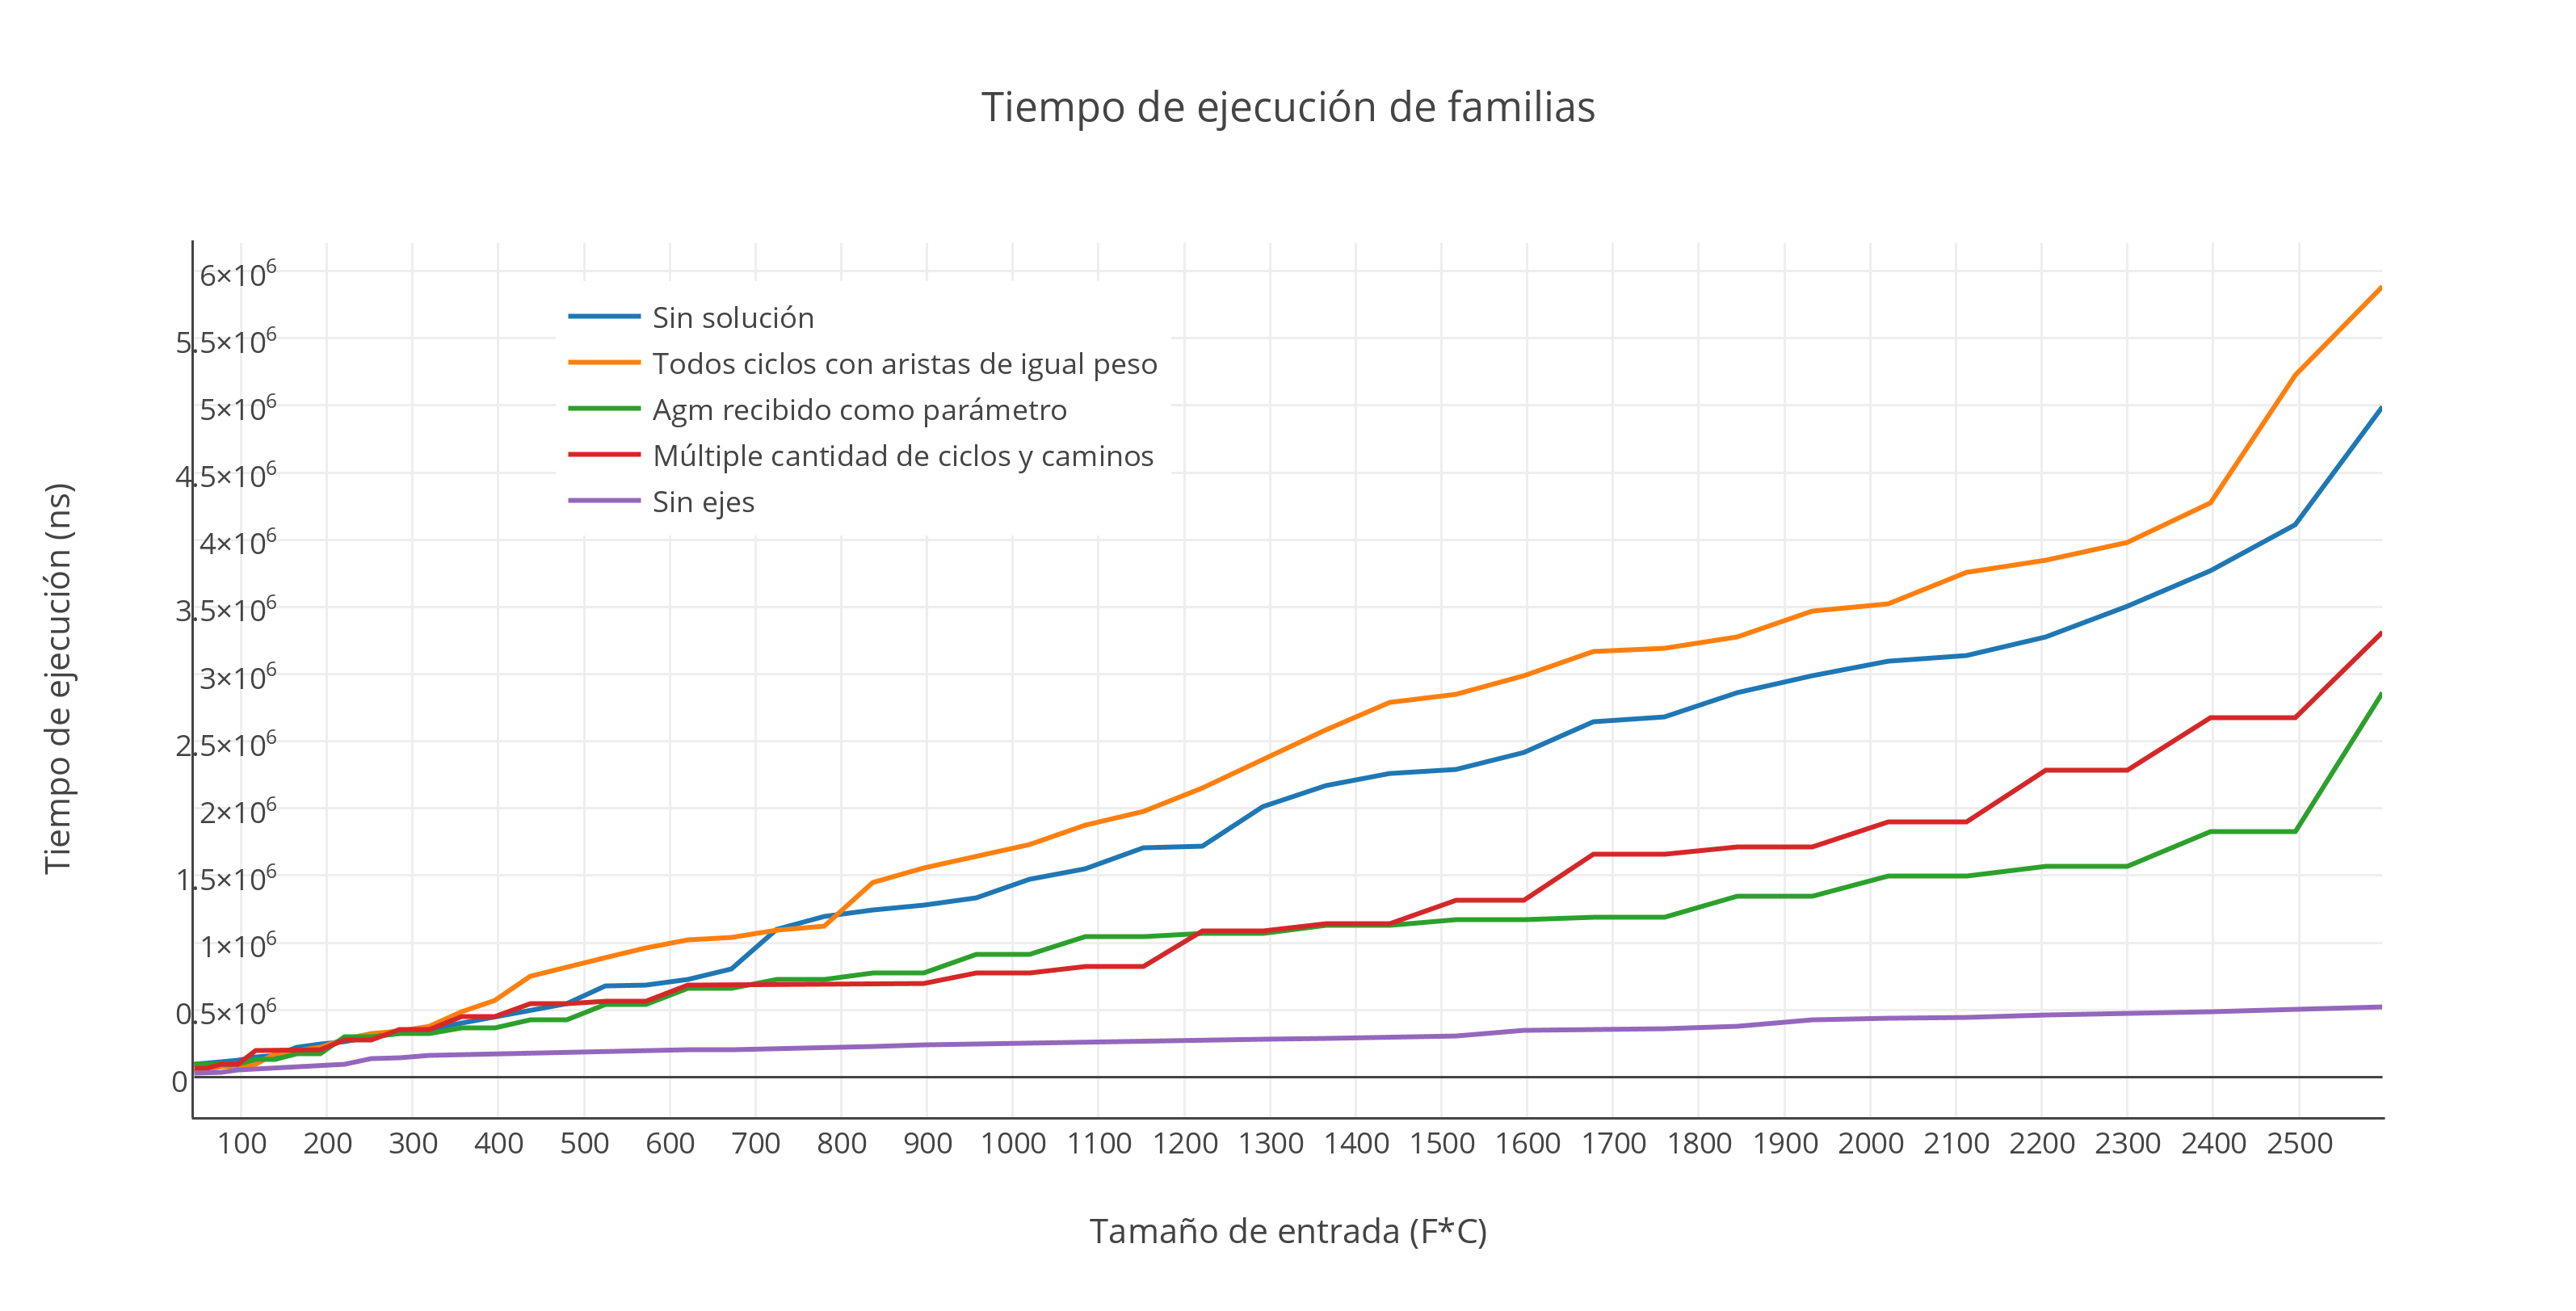
\includegraphics[scale=0.65]{./EJ2/comparativo.png}
 {$Gr$\'a$fico$ \ 2.1 - $Comparativo$}
  \end{center}
  \vspace*{0.3cm}
 

Como se observa en el gr\'afico la funci\'on representativa de la familia 4, presenta una mejor performance en relaci\'on a las otras. Esto se debe a que nuestro algoritmo al intentar chequear las aristas, observa que no hay ninguna y finaliza su ejecuci\'on insumiendo en tiempo unicamente la creaci\'on del grafo (nodos aislados)

Habiendo chequeado dichas instancias, llegamos a la conclusi\'on que la familia de casos que presenta una mejor performance para nuestro algoritmo
es la número 4 dado que el grafo que se obtiene de transformar el laberinto recibido como par\'ametro no presenta ninguna arista.\\

Un grafo representativo de esta familia ser\'ia el siguiente:

\vspace*{0.3cm} \vspace*{0.3cm}
  \begin{center}
 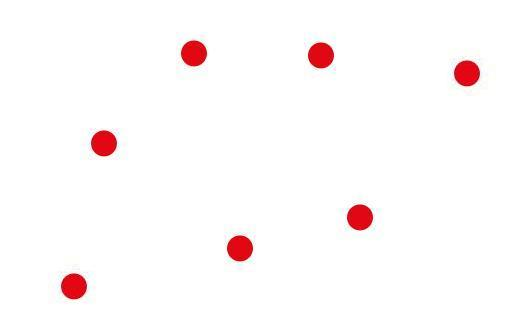
\includegraphics[scale=0.5]{./EJ2/grafoSinEjes.jpeg}
 \\{$Grafo$ \ 2.1 - $Mejor$ $Caso$}
  \end{center}
  \vspace*{0.3cm}

Verificando el peor caso en el gráfico 2.1, llegamos a la conclusi\'on que la familia de casos que hace que el algoritmo tenga más tiempo de cómputo ser\'a la familia 2 dado que el grafo que se obtiene de transformar el laberinto de entrada es aquel que presenta un ciclo por cada habitaci\'on posible, dandonos el siguiente grafo una vez transformado:\\

\vspace*{0.3cm} \vspace*{0.3cm}
  \begin{center}
 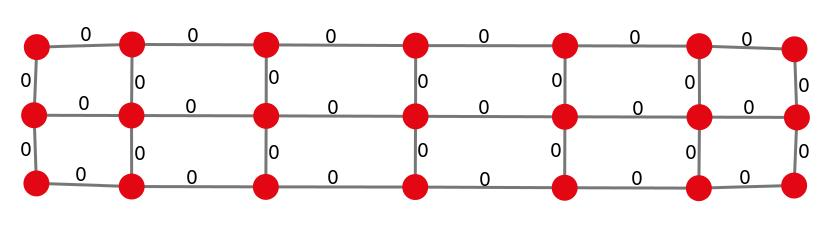
\includegraphics[scale=0.5]{./EJ2/ej2grafosinpared.jpeg}
 \\{$Grafo$ \ 2.2 - $Peor$ $Caso$}
  \end{center}
  \vspace*{0.3cm}

  
Veamos en detalle como se comportan el mejor y peor caso con respecto a la complejidad teorica calculada.\\

\vspace*{0.3cm} \vspace*{0.3cm}
  \begin{center}
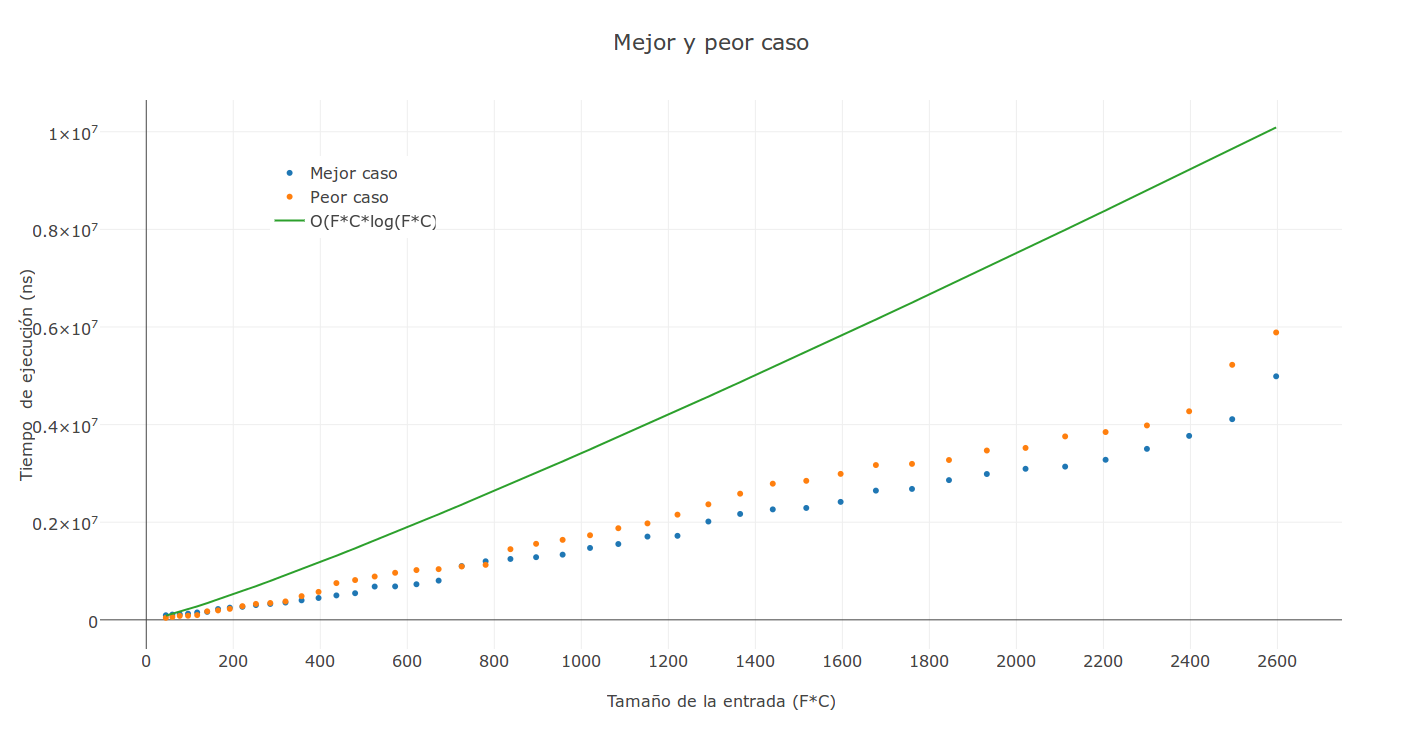
\includegraphics[scale=0.35]{./EJ2/MejorYPeorCaso.png}
 {$Gr$\'a$fico$ \ 2.5 - $Comparativo$}
  \end{center}
  \vspace*{0.3cm}
    
  
Podemos ver como las familias est\'an acotadas por la funci\'on de la complejidad te\'orica calculada.\\
  
Luego de dichos experimentos y casos probados, se puede concluir que a pesar de tener ciclos en todas las salas y donde dichos ciclos presenten aristas con pesos iguales lo que genera al algoritmo la posibilidad de crear varias ramas posibles de soluci\'on los tiempos se mantienen dentro de la complejidad propuesta.\\
